% Bagian Lampiran
\section*{Lampiran} % Jika ada lampiran

% ini buat percobaan 1

\begin{figure}[H]
  \centering
  % Kalau mau menambah gambar lagi tinggal nambahin begin{subfigure} -> end{subfigure}
  \begin{subfigure}[c]{0.4\linewidth}
    \centering
    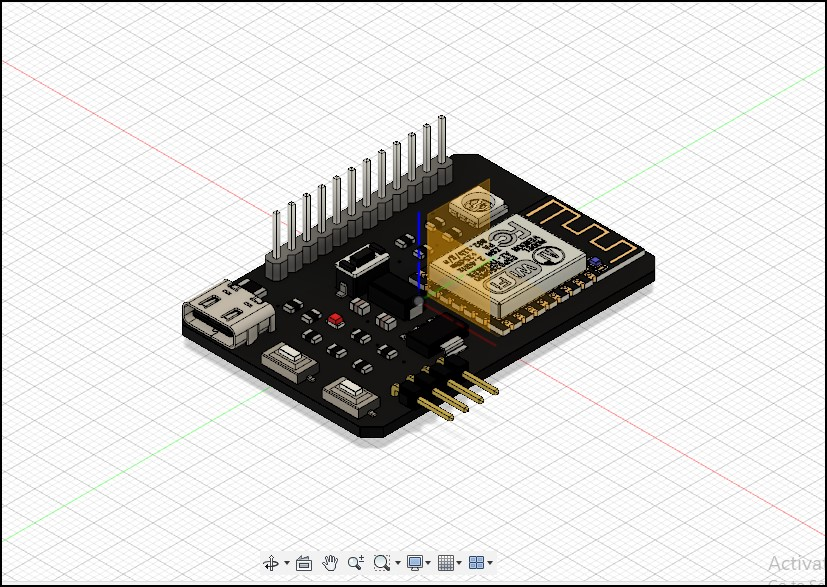
\includegraphics[width=\linewidth]{img/modul_3/file_step_modul_3.jpg}
    \caption{STEP file modul 3\label{fig:inisub1}}
  \end{subfigure}
  \hspace{1cm}
  \begin{subfigure}[c]{0.4\linewidth}
    \centering
    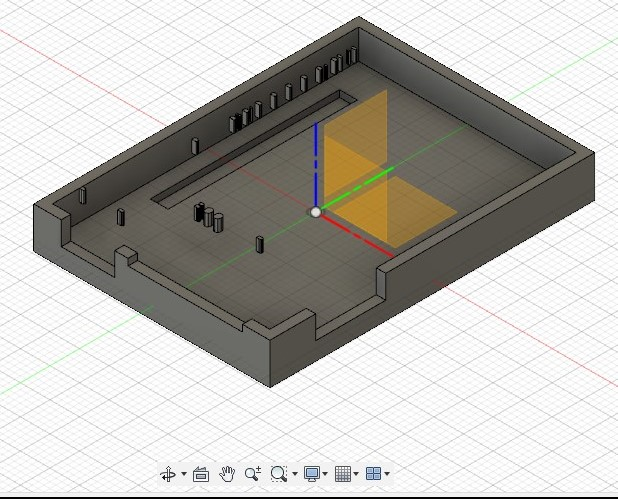
\includegraphics[width=\linewidth]{img/modul_3/enclosure_bawah.jpg}
    \caption{Hasil enclosure bawah \label{fig:inisub2}}
  \end{subfigure}
  \caption{Hasil percobaan 1 \label{fig:keduagambar}}
\end{figure}

\begin{figure}[H]
  \centering
  % Kalau mau menambah gambar lagi tinggal nambahin begin{subfigure} -> end{subfigure}
  \begin{subfigure}[c]{0.4\linewidth}
    \centering
    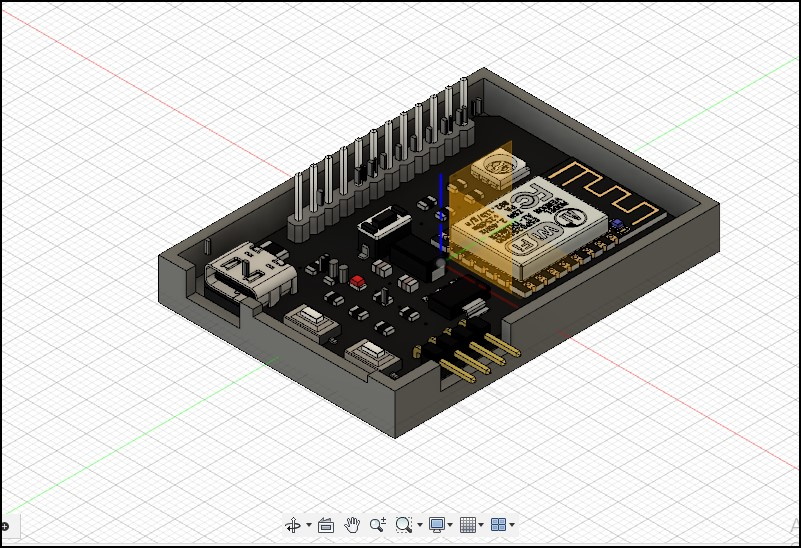
\includegraphics[width=\linewidth]{img/modul_3/enclosure_bawah_withcomponent.jpg}
    \caption{Hasil enclosure bawah dengan komponen \label{fig:inisub1}}
  \end{subfigure}
  \hspace{1cm}
  \begin{subfigure}[c]{0.4\linewidth}
    \centering
    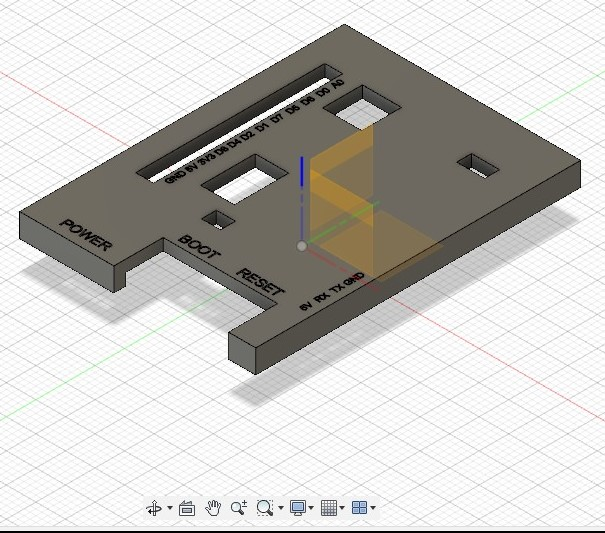
\includegraphics[width=\linewidth]{img/modul_3/enclosure_atas.jpg}
    \caption{Hasil enclosure atas \label{fig:inisub2}}
  \end{subfigure}
\end{figure}

\begin{figure}[H]
  \centering
  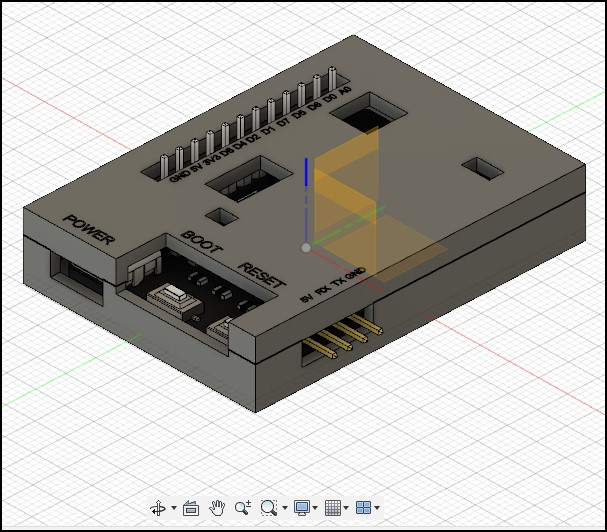
\includegraphics[width=0.6\linewidth]{img/modul_3/enclosure_full_withcomponent.jpg}
  \caption{Hasil enclosure atas dan bawah \label{fig:inisub1}}
\end{figure}

\begin{figure}[H]
  \centering
  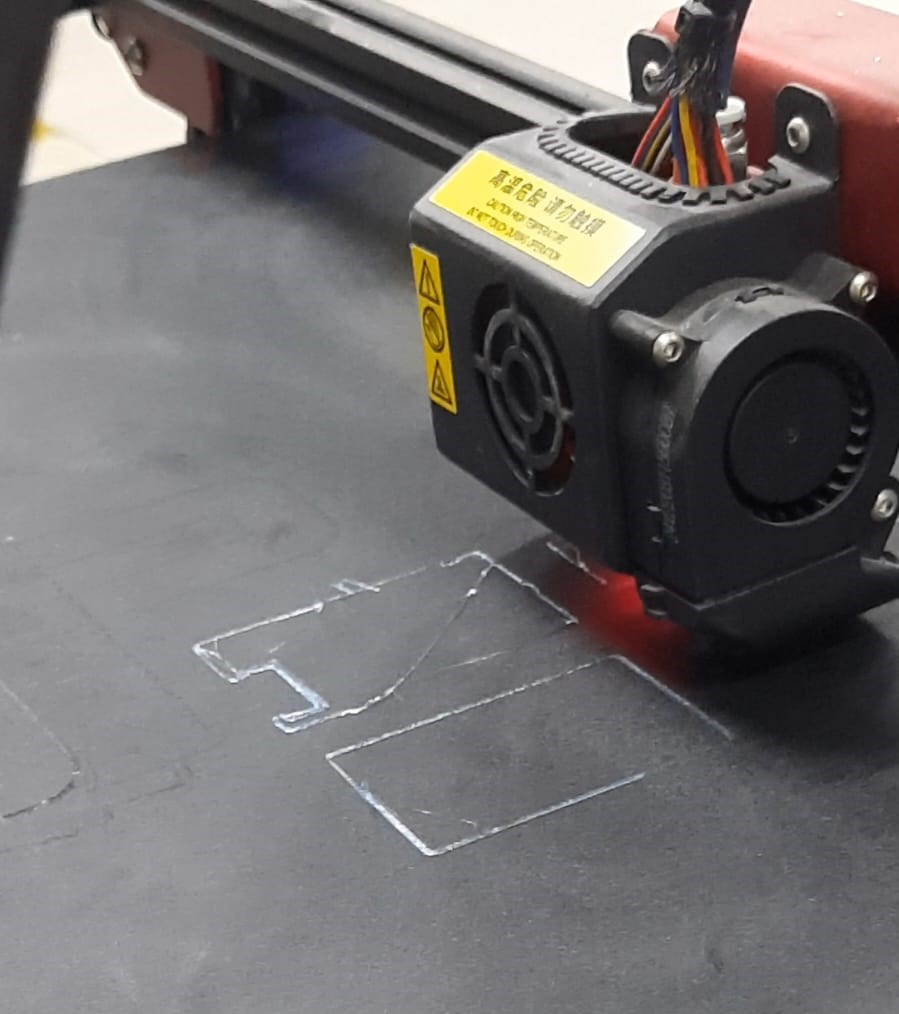
\includegraphics[width=0.6\linewidth]{img/modul_3/proses_3d_printing.jpg}
  \caption{Proses 3D printing \label{fig:inisub1}}
\end{figure}